\documentclass[xcolor=pdftex,dvipsnames]{beamer}
\usepackage{harvard}
\usepackage{amsmath}
\usepackage{amssymb}

\title{Microeconomic Theory --- ECON 323 503 \\ Math Review} 
\author{Vikram Manjunath}
\institute{Texas A\&M University}
\setbeamertemplate{navigation symbols}{}
\setbeamertemplate{footline}{}
\usefonttheme{serif}
\begin{document}

\maketitle

\begin{frame}
\frametitle{Outline}
\begin{enumerate}
\item Real numbers
\item Functions 
\item Lines
\item Derivatives
\item Some properties of functions
\item Functions of more than one variable
\item Partial derivatives
\item Finding the maximum or minimum of a function
\end{enumerate}

\end{frame}

\begin{frame}\frametitle{Real numbers}
\uncover<1->{Real numbers are nearly all of the numbers you'd ever
  think of.}
\bigskip

\uncover<2->{
Real numbers are important in economics because they represent:
\begin{itemize}
\item Amounts of resources
\item Amounts of money
\item Interest rates
\item Probabilities
\item And so many more things
\end{itemize}}
\end{frame}

\begin{frame}\frametitle{Real line}
Real numbers are represented in the real line: they are ordered! 
\bigskip

\uncover<2->
{They get bigger as you move to the right.}

\bigskip
\uncover<3->{
\begin{center}
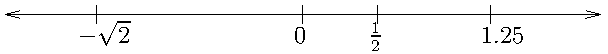
\includegraphics{pics/RealLine}
\end{center}
}
\end{frame}

\begin{frame}\frametitle{Functions of a single variable}

Two sets: $X$ and $Y$ (might be the same)

\bigskip

\uncover<2->{
Function: $f:X\to Y$

Maps every member of $X$ with a member of $Y$.
}\bigskip

\uncover<3->{
We'll represent the member of $Y$ that f maps $x$ to by $f(x)$.
}

\begin{center}
\only<1>{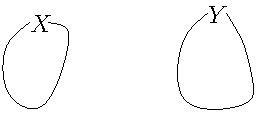
\includegraphics{pics/func1}}
\only<2>{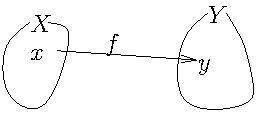
\includegraphics{pics/func2}}
\only<3->{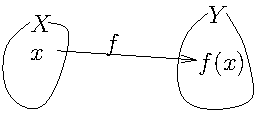
\includegraphics{pics/func3}}
\end{center}
\uncover<4>{For our purposes, $X$ and $Y$ will usually be the real
  numbers ($\mathbb R$).}
\end{frame}




\begin{frame}
\frametitle{Examples of functions}
\begin{itemize}[<+->]
\item Identity: for each $x\in X$, {\color{red}$f(x)=x$}.
\item Constant: for each $x\in X$,{\color{red} $f(x)=c$} where $c$ is fixed.
\item Square root: for each $x\geq 0,$ {\color{red} $f(X) = \sqrt{x}$}.
\item Linear: for each $x\in X$, {\color{red}$f(x) = mx+c$} where $m$ and $c$ are fixed.
\end{itemize}
\end{frame}

\begin{frame}
\frametitle{Lines}
Speaking of linear functions, they describe \emph{lines} (hence the
name).\bigskip

\uncover<2->{
Suppose $m=0.5$ and $c=1$. Then $f(x) = 0.5 x + 1$.\bigskip
}

\only<1,2>{
\vspace{1.95in}
}

\only<3>{
$f(-1) = 0.5\times (-1) + 1 = 0.5$.\bigskip
}
\only<4>{
$f(0) = 0.5\times (0) + 1 = 1$.\bigskip
}
\only<5>{
$f(1) = 0.5\times (1) + 1 = 1.5$.\bigskip
}

\only<6>{
Connect the dots.\bigskip
}
\only<7>{
Now you have a line.\bigskip
}
\begin{center}
\only<3>{
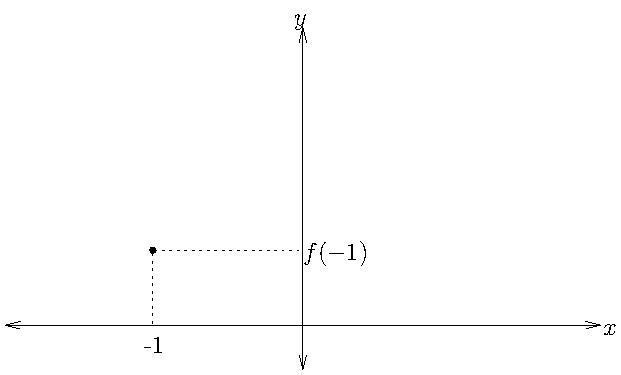
\includegraphics[scale=0.7]{pics/linear1}
}
\only<4>{
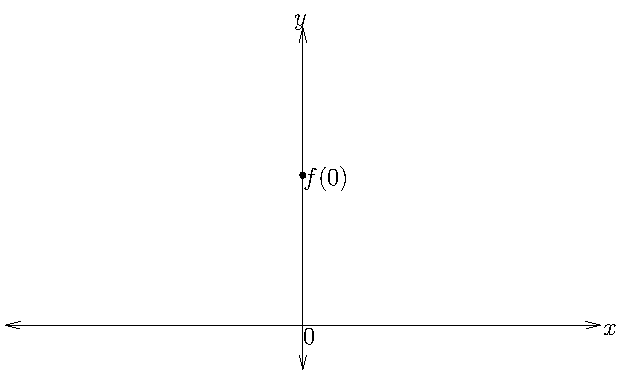
\includegraphics[scale=0.7]{pics/linear2}
}
\only<5>{
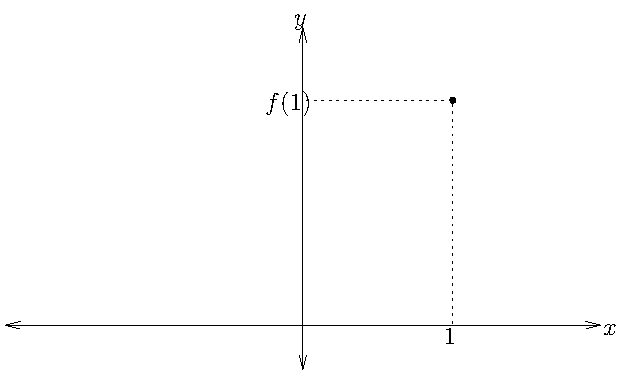
\includegraphics[scale=0.7]{pics/linear3}
}
\only<6>{
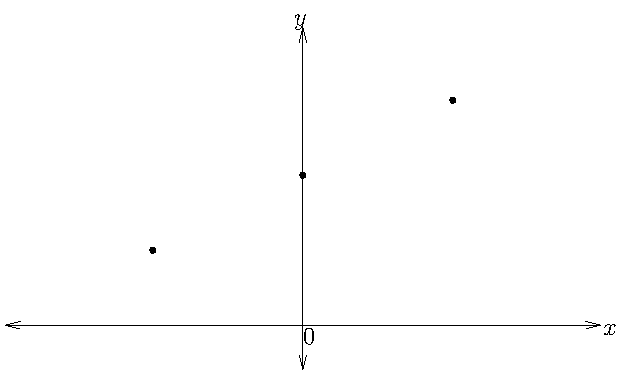
\includegraphics[scale=0.7]{pics/linear4}
}
\only<7>{
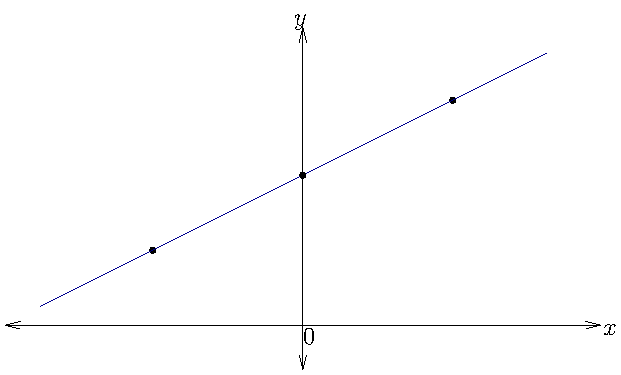
\includegraphics[scale=0.7]{pics/linear5}
}
\end{center}


\end{frame}



\begin{frame}\frametitle{Slope of a line}
We call $m$ the ``slope'' of the line $mx+c$.

That's because for increment in $x$, the value of $mx+c$ increases $m$
times.

\begin{center}
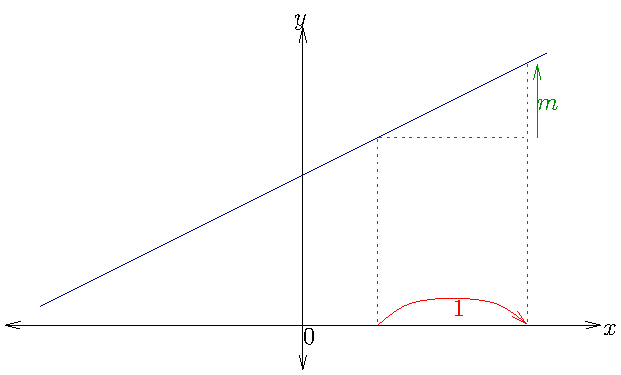
\includegraphics[scale=0.7]{pics/slope}
\end{center}
\end{frame}


\begin{frame}
\frametitle{Slope of a line}
So the slope of a line is the ratio of the change in $f(x)$ to the
change in $x$. Suppose $x$ changes from $x_1$ to $x_2$:
\[
\text{slope } =m=\frac{f(x_2)-f(x_1)}{x_2-x_1}.
\]
\end{frame}


\begin{frame}\frametitle{Graph of a function}
We can draw the ``graph'' of any function in this way, by connecting
the dots representing each $x$ and corresponding $f(x)$.

\begin{center}
\only<1>{
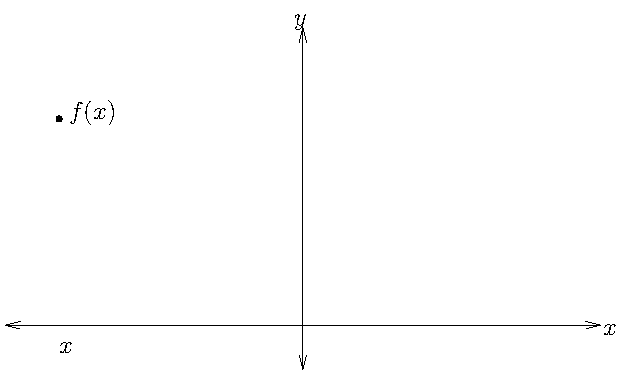
\includegraphics[scale=0.7]{pics/graph1}
}
\only<2>{
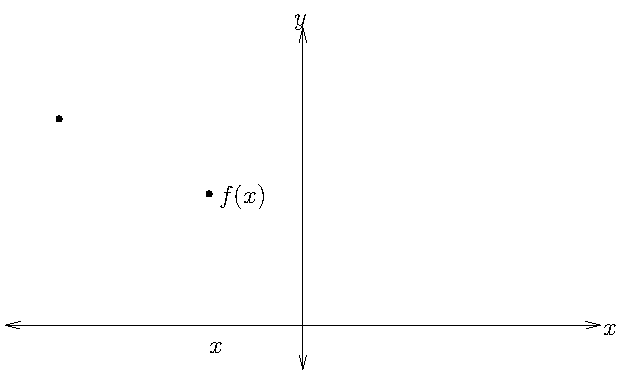
\includegraphics[scale=0.7]{pics/graph2}
}
\only<3>{
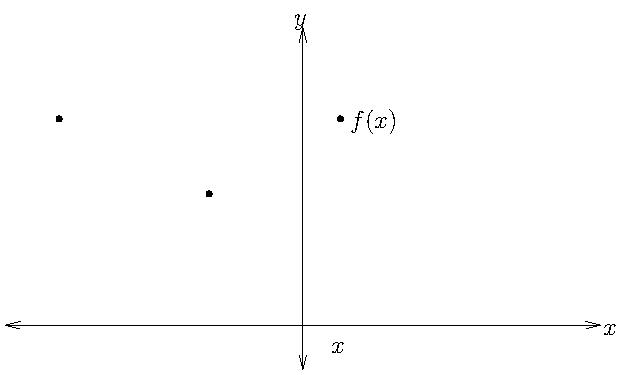
\includegraphics[scale=0.7]{pics/graph3}
}
\only<4>{
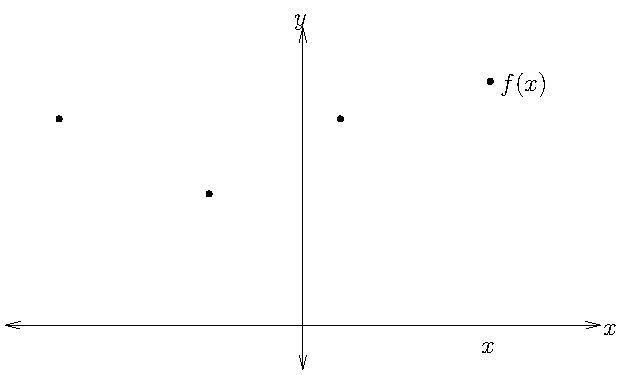
\includegraphics[scale=0.7]{pics/graph4}
}
\only<5>{
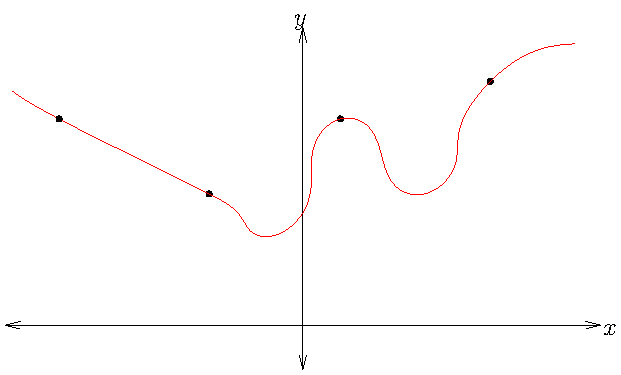
\includegraphics[scale=0.7]{pics/graph5}
}
\end{center}


\end{frame}


\begin{frame}
\frametitle{Derivative of a function}

\only<1>{Recall the slope of a line is $\frac{f(x_2)-f(x_1)}{x_2-x_1}.$ It
doesn't depend on how far apart or where  $x_1$ and $x_2$ are.}
\bigskip

\only<2>{
If $f$ isn't linear, it will. So what is the slope of $f$? It's the
same thing where the change in $x$ is as small as possible.
}
\bigskip

\only<3>{
So, if $x$ changes from $x$ to $x+h$, the ratio of the change in
$f(x)$ to the change in $x$ is just 
\[\frac{f(x+h) - f(x)}{(x+h) - x} = \frac{f(x+h)- f(x)}{h}.
\]
}

\only<4>{
To make $h$ \emph{as small as possible}, we take the limit as $h$ goes
to zero:
\[
\lim_{h\to 0}\frac{f(x+h) - f(x)}{h}.
\]

\bigskip
\begin{center}{\small (Don't let the $\lim_{h\to 0}$ scare you... )}\end{center}
}

\only<5>{
We'll represent this with the notation $\frac{df(x)}{dx}$.
}

\end{frame}


\begin{frame}
\frametitle{Geometrically}
\begin{center}
\only<1>{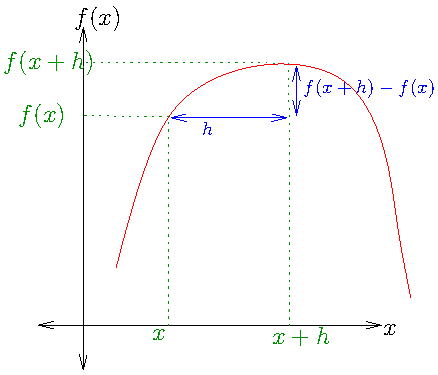
\includegraphics{pics/Deriv1}}
\only<2>{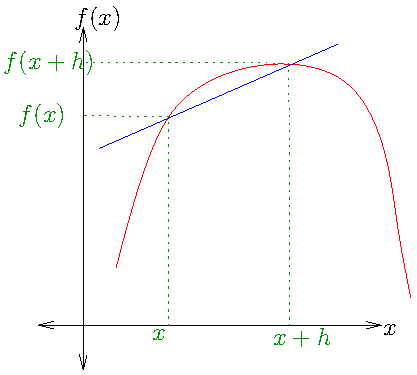
\includegraphics{pics/Deriv2}}
\only<3>{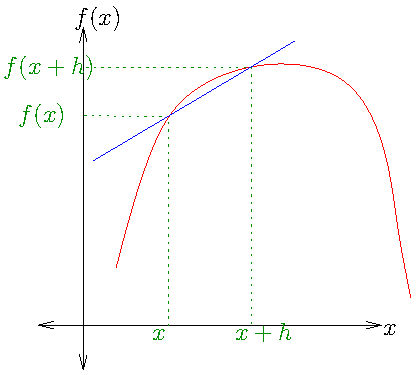
\includegraphics{pics/Deriv3}}
\only<4>{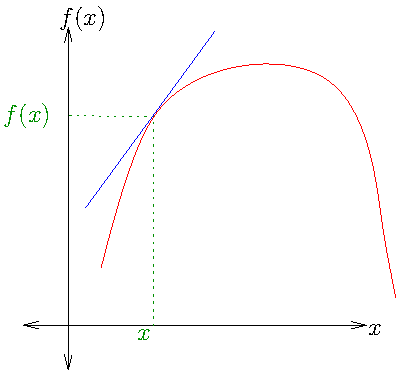
\includegraphics{pics/Deriv4}}
\only<5>{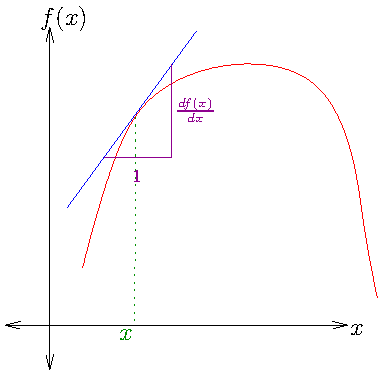
\includegraphics{pics/Deriv5}}
\end{center}
\end{frame}




\begin{frame}
\frametitle{Some basic rules to calculate derivatives}
\begin{enumerate}
\uncover<1>{\item Constant: If $f(x) = c$ then $\frac{df(x)}{dx} =0$.}
\uncover<2>{\item Addition: If $f(x) = g(x) + h(x)$ then 
\[
\frac{df(x)}{dx} = \frac{dg(x)}{dx} + \frac{dh(x)}{dx}.
\]}
\uncover<3>{
\item Multiplication: If $f(x) = g(x)h(x)$ then 
\[
\frac{df(x)}{dx} = \frac{dg(x)}{dx}h(x) + g(x)\frac{dh(x)}{dx}.
\]
}
\uncover<4>{
\item Power: If $f(x) = ax^b$ then
\[
\frac{df(x)}{dx} = abx^{b-1}.
\]
}
\uncover<5>{
\item Logarithm: If $f(x) = ln(x)$ then
\[
\frac{df(x)}{dx} = \frac{1}{x}.
\]
}
\end{enumerate}
\end{frame}

\begin{frame}
\frametitle{Some basic rules to calculate derivatives}
\begin{enumerate}
\item[6.] Chain: If $f(x) = g(h(x))$ then 
\[
\frac{df(x)}{dx} = \frac{dg(h(x))}{dh(x)}\frac{dh(x)}{dx}
\]\end{enumerate}

\end{frame}


\begin{frame}
\frametitle{Derivatives of more complicated functions?}
You can use the basic rules as building blocks to take derivatives of
many functions (and all of the ones that we'll see in this class).
\end{frame}



\begin{frame}
\frametitle{An example}

\[f(x) = 5x^4+xln(x)
\]
\begin{enumerate}
\item<2,3,4,8>
 addition rule with $g(x) = 5x^4$ and $h(x)=xln(x)$\bigskip
\item <3,8>
$\frac{dg(x)}{dx} = 5\times 4x^{4-1} = 20x^3$.
\item<4,5,6,7>
What's $\frac{dh(x)}{dx}$? We need the product rule for $h(x) = g'(x)h'(x)$ with $g'(x) = x$
and $h'(x) = ln(x)$.
\item <5,7> $\frac{dg'(x)}{dx} = 1$.
\item<6,7> $\frac{dh'(x)}{dx} = \frac{1}{x}$.
\item<7,8> Putting these two together, using the product rule, 
\[\frac{dh(x)}{dx} = \frac{dg'(x)}{dx}h'(x) + g'(x) \frac{dh'(x)}{dx} =
1ln(x) + x\frac{1}{x} = ln(x)+1.
\]
\item<8>Finally, using the addition rule
\[
\frac{df(x)}{dx} = \frac{dg(x)}{dx} +\frac{dh(x)}{dx} = 20x^3 + ln(x)
+ 1.
\]
\end{enumerate}



\end{frame}
\begin{frame}
\frametitle{Another example}
\[f(x) =  \frac{1}{3}\left(x-\frac{1}{2}\right)^3
\]
\uncover<2->{Use the chain rule for $f(x) = g(h(x))$ where $g(y) =
  \frac{1}{3}y^3$ and $h(x) = x-\frac{1}{2}$.}\bigskip

\uncover<3->{
$\frac{dg(y)}{dy} = y^2.$\bigskip
}

\uncover<4->{
$\frac{dh(x)}{dx} = 1.$\bigskip
}

\uncover<5->{ Using the chain rule, 
\[
\frac{df(x)}{dx} = \frac{dg(h(x))}{dh(x)}\frac{dh(x)}{dx} =
(h(x))^2\times 1 = \left(x-\frac{1}{2}\right)^2.
\]
}

\end{frame}
\begin{frame}
\frametitle{Some properties of functions}
\begin{enumerate}
\item Monotonicity
\item Continuity
\item Concavity
\item Convexity
\end{enumerate}
\end{frame}




\begin{frame}
\frametitle{Monotonicity}

The function is either always going up or always going down as you
move $x$ in the same direction.\bigskip

\only<1>{This function is monotonic:

\begin{center}
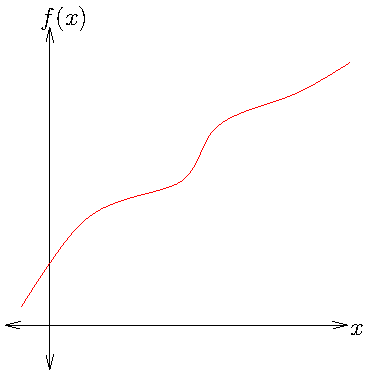
\includegraphics{pics/monotonic}
\end{center}
}


\only<2>{
This function is \emph{not} monotonic

\begin{center}
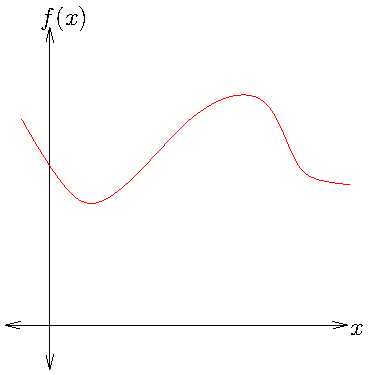
\includegraphics{pics/nonmonotonic}
\end{center}
}
\end{frame}


\begin{frame}
\frametitle{Continuity}

The graph of the function doesn't ``jump'' or have any ``breaks'' in
it.


\only<1>{This function is continuous:

\begin{center}
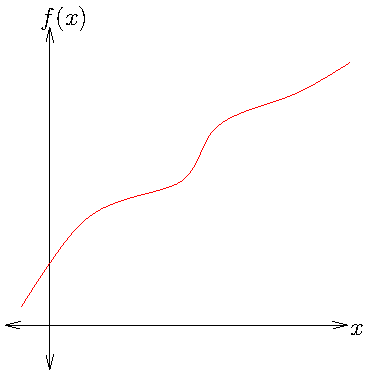
\includegraphics{pics/monotonic}
\end{center}
}


\only<2>{
This function is \emph{not} continuous

\begin{center}
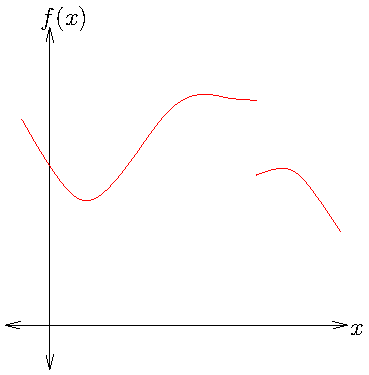
\includegraphics{pics/discontinous}
\end{center}
}


\end{frame}


\begin{frame}
\frametitle{Concavity}
What can we say about this derivative of this function as $x$ moves to
the right?
\begin{center}
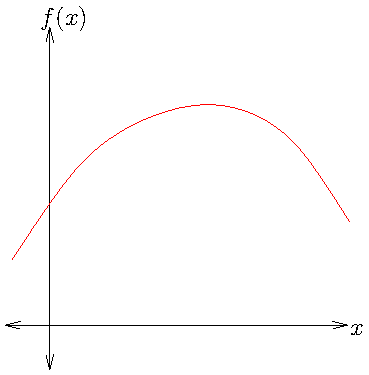
\includegraphics{pics/concave}
\end{center}
\uncover<2>{
It's decreasing.
}
\end{frame}



\begin{frame}
\frametitle{Convexity}
What can we say about this derivative of this function as $x$ moves to
the right?
\begin{center}
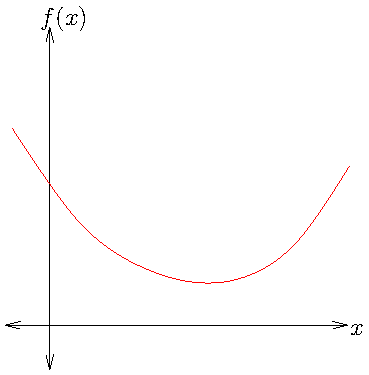
\includegraphics{pics/convex}
\end{center}
\uncover<2>{
It's increasing.
}
\end{frame}


\begin{frame}
\frametitle{Concavity and convexity}
This function is neither concave nor convex.

\begin{center}
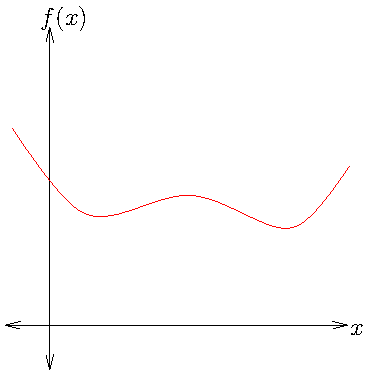
\includegraphics{pics/nonconvexconcave}
\end{center}


\end{frame}

\begin{frame}
\frametitle{Concavity and convexity}
We see a lot of functions like this in economics.\bigskip

\uncover<2->{Why do economists like them so much?}\bigskip

\uncover<3->{Because we can find the ``maximum'' of a concave function
  and the ``minimum'' of a convex function.}

\uncover<4->{\begin{center}
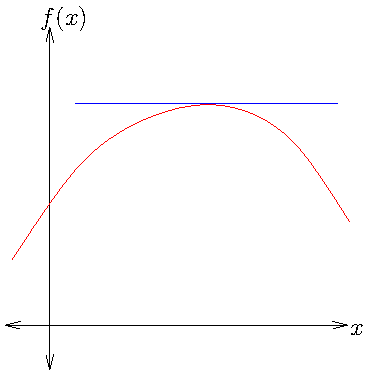
\includegraphics[scale=0.6]{pics/Max}
\end{center}}


\uncover<5->{We just have to find the spot where the derivative is
  zero. For a concave function, it's flat at the very top of the hill
  and for a convex function, it's flat at the very bottom of the valley}

\end{frame}


\begin{frame}
\frametitle{Functions of more than one variable}

\begin{enumerate}[<+->]
\item $f$ may map \emph{pairs} of members of $X$ with members of
  $Y$. Then $f:X^2\to Y$. We write $f(x_1,x_2)$ to denote the value
  that the pair $(x_1,x_2)$ is mapped to.
\item $f$ may map \emph{triples}\dots\\
We write $f(x_1,x_2,x_3)$\dots
\item \dots
\item \dots $f(x_1,x_2,\dots,x_n)$\dots
\end{enumerate}
\end{frame}

\begin{frame}
\frametitle{How do you graph a function of two variables?}
You need three dimensions to do that.

\uncover<2->{
\begin{center}
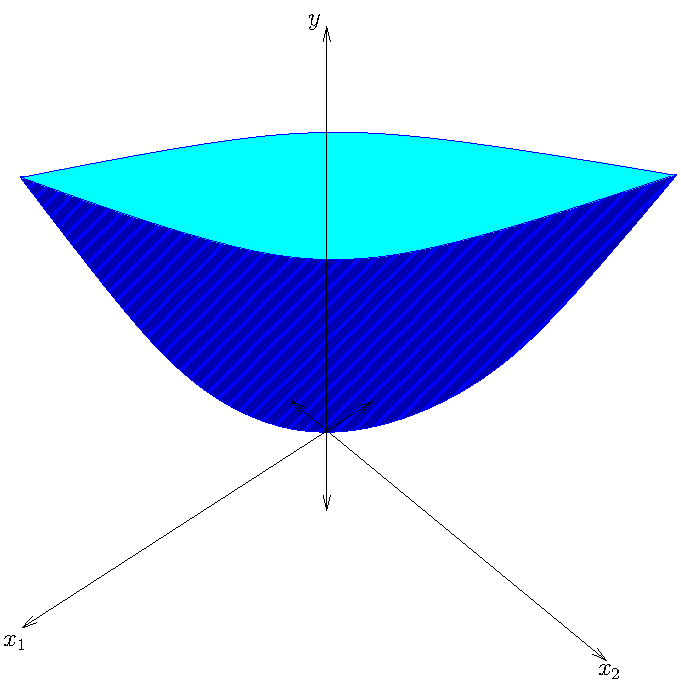
\includegraphics[scale=0.6]{pics/3d}\end{center}
}
\end{frame}

\begin{frame}
\frametitle{What about three variables?}
Now you need four dimensions\dots
\end{frame}


\begin{frame}
\frametitle{An easier way to visualize functions of two variables}
Just like a topographic map, we just draw a curve through all the
pairs $(x_1,x_2)$ that are mapped to the same value.

\only<1>{Suppose $f({\color{red}x_1,x_2}) = y$.
\begin{center}
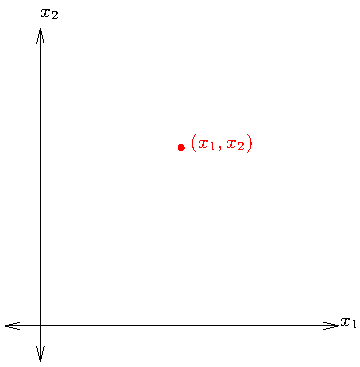
\includegraphics{pics/level1}
\end{center}
}
\only<2>{And $f({\color{blue}x_1',x_2'}) = y$ too.
\begin{center}
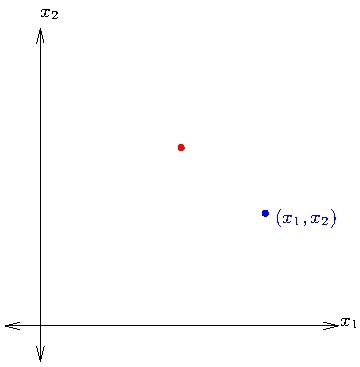
\includegraphics{pics/lev2}
\end{center}
}
\only<3>{Find all such pairs.
\begin{center}
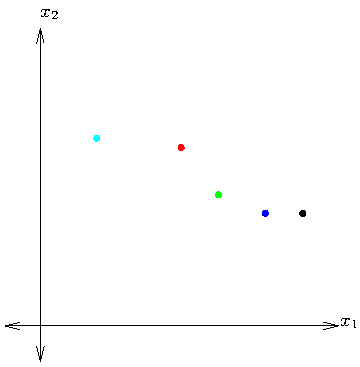
\includegraphics{pics/lev3}
\end{center}
}
\only<4>{Find all such pairs.
\begin{center}
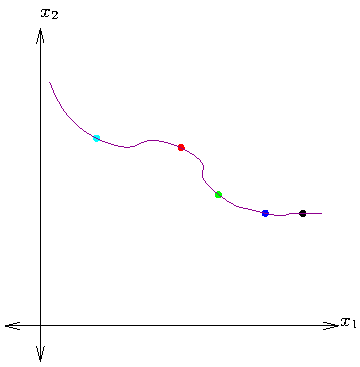
\includegraphics{pics/lev4}
\end{center}
}

\uncover<4>{This is a ``iso-level set'' of $f$.}


\end{frame}


\begin{frame}
\frametitle{Partial derivatives}
A \emph{partial derivative} is the derivative when you hold one of the ``arguments'' fixed. \bigskip

\uncover<2->{Suppose $f:\mathbb R^2\to \mathbb R$.

To find the partial derivative of $f$  with respect to $x_1$, treat
$x_2$ as a constant. (Of course, this means that the partial
derivative is different for different $x_2$.)\bigskip
}

\uncover<3->{We write $\frac{\delta f(x_1,x_2)}{\delta x_1}$ to
  represent the partial derivative of $f$ with respect to $x_1$.
}

\end{frame}


\begin{frame}
\frametitle{An example}

\[
f(x_1,x_2) = x_1^2 + x_2^2 + 2x_1x_2
\]

\uncover<2->{Just take the derivative, treating $x_2$ as a constant:

\[\frac{\delta f(x_1,x_2)}{\delta x_1} = 2x_1 + 0 + 2x_2 = 2x_1 + 2x_2.
\]
}



\end{frame}

\begin{frame}
\frametitle{Finding the maximum or minimum of a function}
We'll talk about maximizing a function (minimizing is essentially
the same thing). So let's suppose that our functions are concave.\bigskip

\uncover<2->{
Think of climbing a hill. At the very top, it's flat. So we need to
look for the argument where no changes to the argument can cause
an increase in the function's value.\bigskip
}

\uncover<3->{
The maximum of $f:\mathbb R\to \mathbb R$ is
\[
\max_x f(x).
\]
}

\uncover<4->{
To find it, solve for $x$ such that $\frac{df(x)}{dx} = 0$.
}
\end{frame}

\begin{frame}
\frametitle{An example}
\[
\max_x \frac{1}{2}\left(x-\frac{1}{2}\right)^2
\]
$\frac{df(x)}{dx} = x-\frac{1}{2}$.
\bigskip

\uncover<2->{
Setting $\frac{df(x)}{dx} = x-\frac{1}{2} = 0$, we find that
$x^*=\frac{1}{2}$.\footnote{We denote the ``optimal value of $x$'' by $x^*$.}
}
\end{frame}


\begin{frame}
\frametitle{What about functions of two variables?}
\[\max_{x_1,x_2}f(x_1,x_2)\]
\uncover<2->{
The if the partial derivative with respect to $x_1$ is zero, then a
tiny change in $x_1$ doesn't change the value of the
function. }\bigskip

\uncover<3->{
The same goes for $x_2$.
}\bigskip

\uncover<4->{
So to find $(x_1,x_2)$ where $f(x_1,x_2)$ is maximal, we need two
things to be true:
}
\uncover<5->{
\[
\begin{array}{rcl}
\frac{\delta f(x_1,x_2)}{\delta x_1} &=&0\\
\frac{\delta f(x_1,x_2)}{\delta x_2} &=&0\\
\end{array}
\]
}
\uncover<6->{
These are the ``first order conditions'' for our maximization problem.
}
\end{frame}
\begin{frame}
\frametitle{An example}
\[
\max_{x_1,x_2}\ \frac{1}{2}(x_1 - 4)^2 + \frac{1}{2}(x_2-9)^2
\]
\uncover<2->{FOCs:
\[
\begin{array}{rcccl}
\frac{\delta f(x_1,x_2)}{\delta x_1} &=&  x_1-4   &=& 0\\
\frac{\delta f(x_1,x_2)}{\delta x_2} &=& x_2-9   &=& 0\\
\end{array}
\]}
\uncover<3->{Solve these two equations and you find that $x_1^* = 4$ and
  $x_2^* = 9$.}


\end{frame}


\begin{frame}
\frametitle{Constraints}
You can't always just pick any old $x_1$ and $x_2$. In most economic
problems, we have constraints: if you have \$10, apples cost \$1 each
and bananas cost \$2 each, you can't buy 15 apples and 20 bananas.

\end{frame}
\begin{frame}
\frametitle{Constraints}
Suppose that the constraint is in the form of some function $h$:
\[
\begin{array}{c}\max f(x_1,x_2)\\
\text{s.t. }h(x_1,x_2) = z.
\end{array}
\]
\uncover<2->{The easiest way to deal with this is to use the equation $h(x_1,x_2) =
z$ and solve for $x_2$ in terms of $x_1$. }\bigskip

\uncover<3->{If this leaves us with $x_2 = r(x_1)$, then we really
  have to solve the \emph{unconstrained } problem
\[
\max_{x_1} f(x_1,r(x_1))
\]}

\uncover<4->{This ``substitution method'' doesn't always work. But
  it'll do for most things that we'll see in this course.}

\uncover<5->{When we get to the point where we need a more
  sophisticated method (the Lagrange method), we'll go over that.}

\end{frame}

\begin{frame}
\frametitle{An example}
\[
\begin{array}{c}\max ln(x_1x_2)\\
\text{s.t. }x_1+x_2 = z.
\end{array}
\]
\uncover<2->{
Solving $x_1+x_2=z$ for $x_2$ in terms of $x_1$, we find that $x_2 = z-x_1$.\bigskip
}

\uncover<3->{
Substituting, $ln(x_1x_2) = ln(x_1(z-x_1))$. 
 }\bigskip

\uncover<4->{
So we actually have to solve the \emph{ unconstrained} problem
\[
\max_{x_1} ln(x_1(z-x_1))
\]}

\uncover<5->{
The FOC is:
\[
\frac{1}{x_1} - \frac{1}{z-x_1} = 0.
\]
}

\uncover<6->{
So we find that $x_1^*=\frac{z}{2}$.}\bigskip

\uncover<7->{Use this to find that $x_2^*=z-x_1^* = \frac{z}{2}$.}

\end{frame}

\end{document}






